\section{Machine Learning}

\begin{itemize}
\item What is machine learning?
\item Supervised learning, i.e.\ have labelled data.
\item Binary classification tasks: Every training example has a label indicating
  the class membership.
\item In HEP, the positive class is typically referred to as \emph{signal} while
  the negative class is referred to as \emph{background}.
\item What is training data, etc.
\item What is training.
\end{itemize}


\subsection{Boosted Decision Trees}

Boosted decision trees (BDT) are a classification algorithm consisting on an
ensemble of \emph{decision trees} that are combined to yield a powerful
classifier. The ensemble of decision trees is created using a algorithm referred
to as \emph{boosting}, which iteratively constructs decision tree classifiers or
regressors while emphasising training examples that were incorrectly classified
in prior iterations. The following description of BDT focuses on the algorithm
implemented in \textsc{TMVA}~\cite{TMVA}, which is used in this thesis for the
training of BDTs.

\subsubsection{Classification and Regression Trees}

Classification and regression trees~\cite{Breiman:1984jka,hastie09}, hereafter
collectively referred to as \emph{decision trees}, are used as base functions in
BDTs. A decision tree partitions a multivariate space with coordinates
$\myvec{x} = (x_1, \dots, x_n)$ by recursively performing binary splits along
the coordinate axes until a stopping criterion is met. The resulting binary tree
structure and partitioning is illustrated in \Cref{fig:decision_tree} for a
two-dimensional example. A decision tree with $J$~leaf nodes partitions the
input space into $J$~disjoint subregions denoted by $R_j$ for $j = 1, \dots,
J$. A constant value $c_j$ is assigned to every region $R_j$ such that the
prediction of a decision tree can be written as~\cite{hastie09}
\begin{align*}
  f(\myvec{x}) = \sum_{j = 1}^{J} c_j \, \mathbf{1}(\myvec{x} \in R_j) \qquad \text{with} \qquad \mathbf{1}(\myvec{x} \in R_j) =
  \begin{cases}
    1, & \myvec{x} \in R_j \\
    0, & \text{else}
  \end{cases} \,\text{.}
\end{align*}

\begin{figure}[htbp]
  \centering

  \begin{subfigure}[b]{0.46\textwidth}
    \centering
    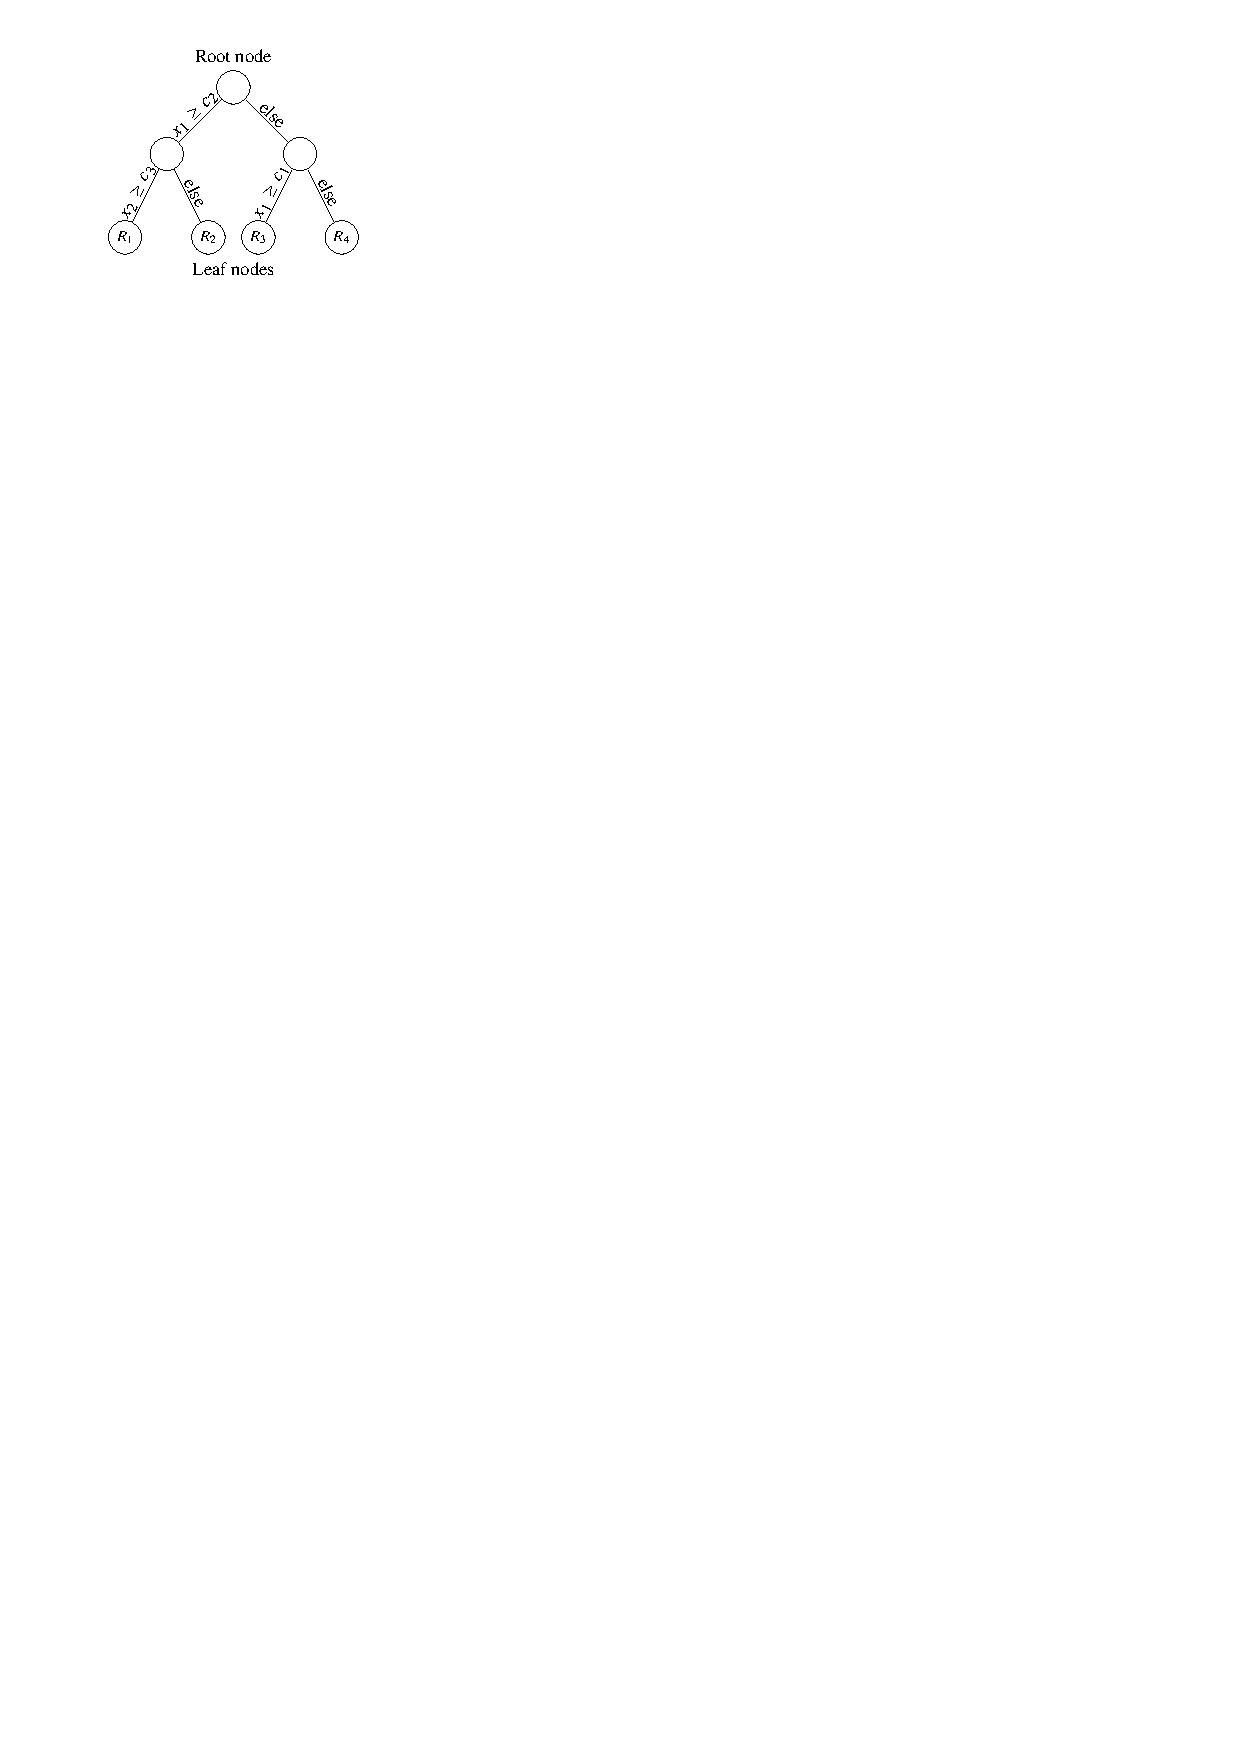
\includegraphics[scale=1.05]{ml/decision_tree}
    \caption{Binary tree structure of a decision tree.}
  \end{subfigure}\hfill%
  \begin{subfigure}[b]{0.46\textwidth}
    \centering
    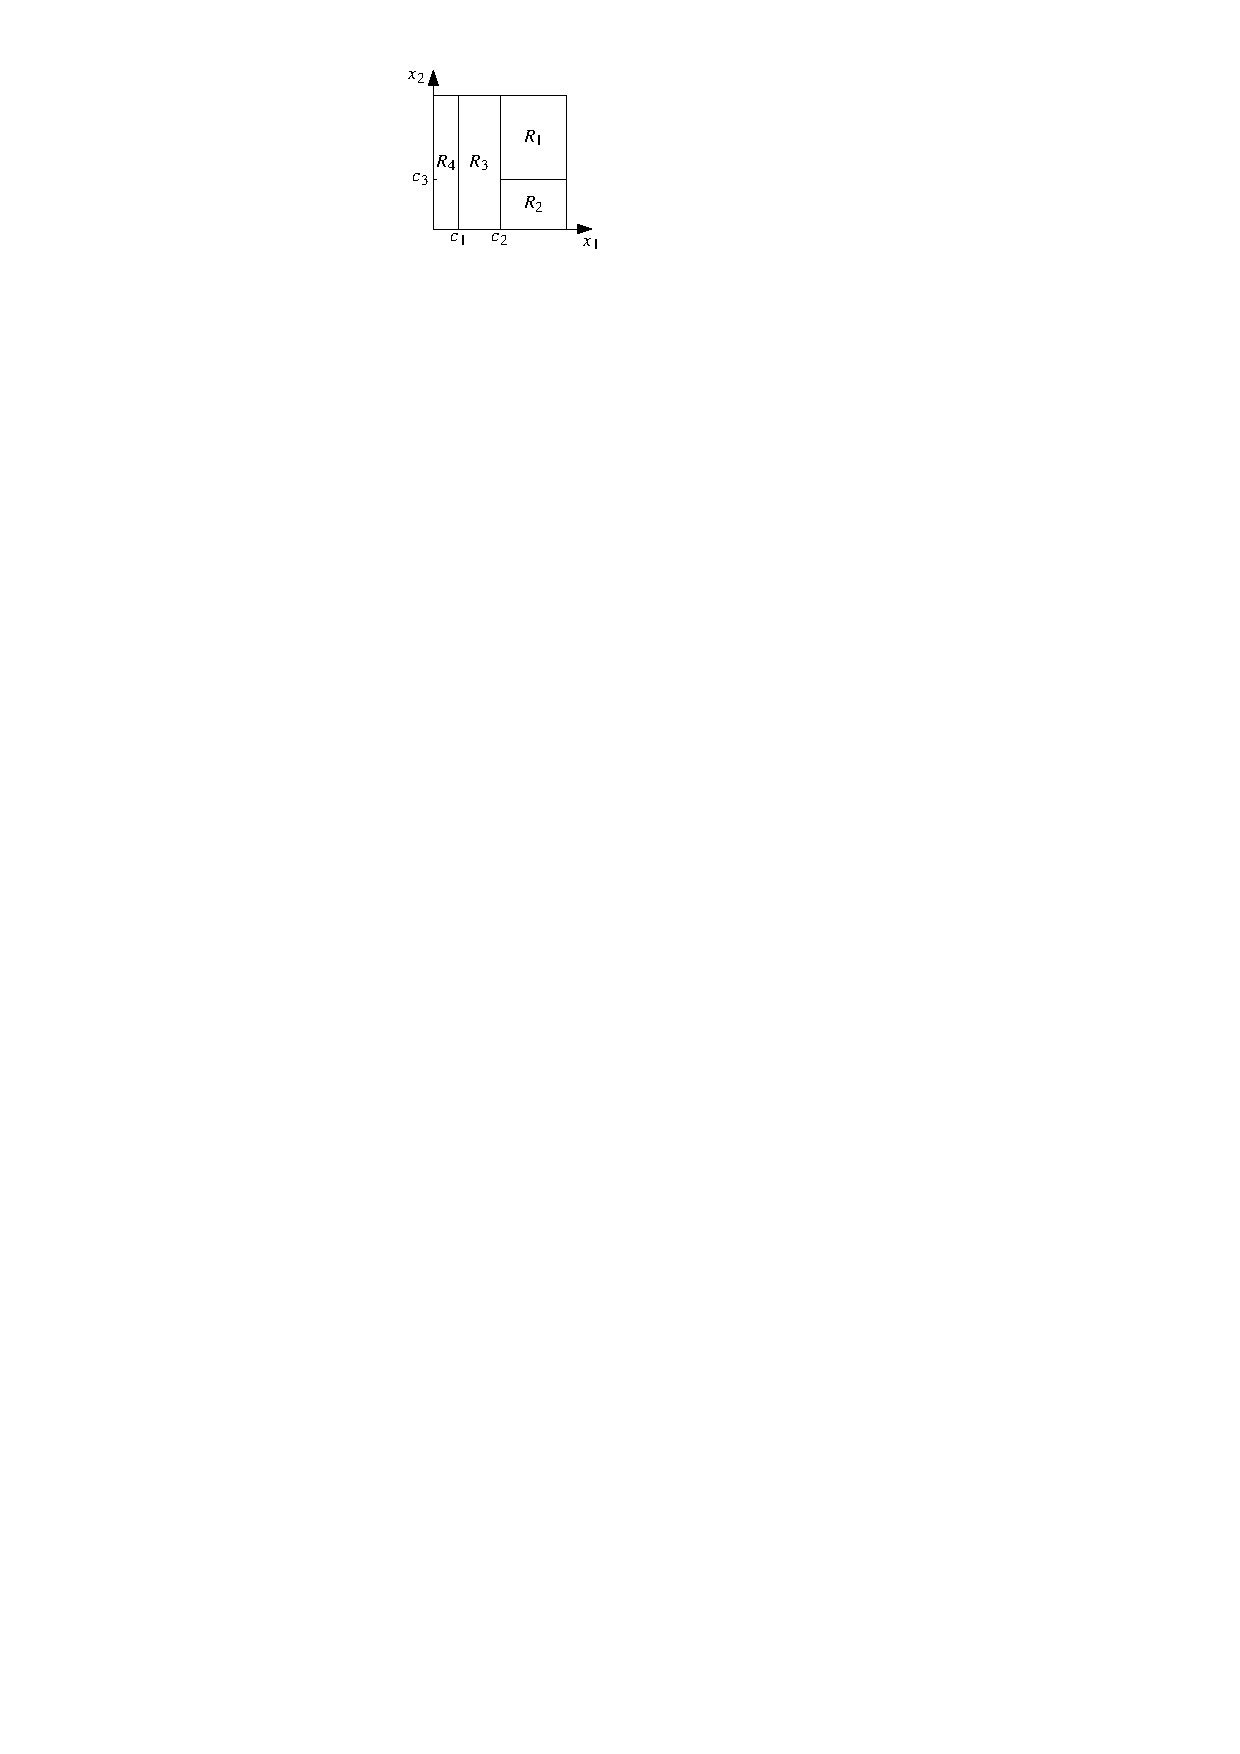
\includegraphics[scale=1.05]{ml/decision_tree_partitioning}
    \vspace*{0.7em}
    \caption{Partitioning resulting from the binary tree in (a).}
  \end{subfigure}\hfill%

  \caption{Example of a decision tree in a two-dimensional space with
    coordinates $\myvec{x} = (x_1, x_2)$. The tree has a depth of two and has
    four leaf nodes that define the regions $R_1, \dots, R_4$. The figure is
    adapted from Ref.~\cite{hastie09}.}%
  \label{fig:decision_tree}
\end{figure}

Classification trees are constructed such that the partitioning of the input
space yields subregions with low impurity, that is, the regions are mostly
populated by training examples of a single class. In this case, the impurity of
a tree node is quantified by the Gini index
\begin{align*}
  I_{\text{G}}(p) = 2 p (1 - p) \,\text{,}
\end{align*}
where $p$ is the proportion of examples from the positive class in a given
node~\cite{hastie09}. A \emph{greedy} strategy is adopted to grow decision trees
by performing the best possible split at every node. This split is determined by
minimising the weighted sum of Gini impurities of the resulting daughter nodes,
where impurities are weighted according to the total weight of training examples
populating a given node. In the classification case, the constants $c_j$
assigned to leaf nodes of the tree are either--depending on the algorithm
configuration--the proportion of examples from the positive class or the class
label of the majority class in a given leaf node.

Regression trees are constructed using a similar approach, however, with an
altered splitting criterion and different assigment of constants to leaf
nodes. Consider the split of a parent node into a left (L) and right (R)
daughter node. Let $(y, w)$ denote the tuple of regression target and weight for
a given training example. Moreover, let $T_{\text{L}}$ and $T_{\text{R}}$ denote
the set of $(y, w)$ for training examples populating the left and right daughter
node, respectively. The constants $c_{\text{L}}$ and $c_{\text{R}}$ assigned to
the daughter nodes are given by
\begin{align*}
  c_{\text{L}} = \frac{\sum_{(y, w) \in T_{\text{L}}} w y}{\sum_{(y, w) \in T_{\text{L}}} w} \qquad \text{and} \qquad c_{\text{R}} = \frac{\sum_{(y, w) \in T_{\text{R}}} w y}{\sum_{(y, w) \in T_{\text{R}}} w} \,\text{,}
\end{align*}
which is the weighted mean of the regression target for the training examples
populating the left and right node, respectively. The best possible split in a
regression tree is chosen such that the squared error defined as
\begin{align*}
  \sum_{(y, w) \in T_{\text{L}}} w (y - c_{\text{L}})^2 + \sum_{(y, w) \in T_{\text{R}} } w (y - c_{\text{R}})^2
\end{align*}
is minimised.


\subsubsection{Boosting of Decision Trees}

Boosting is a meta-learning algorithm...

% construct an additive model
% \begin{align*}
%   F(x) = \sum_{m = 1}^{M} \beta_m b(x; \gamma_m) \,\text{,}
% \end{align*}
% where $b(x; \gamma_m)$

\textsc{AdaBoost}~\cite{freund_shapire:adaboost,freund_shapire:adaboost2} and
more general gradient boosting techniques that allow to minimise an arbitrary
differentiable loss function.  In this thesis, the gradient boosting
implementation of TMVA~\cite{TMVA} is used which implements the
\textsc{TreeBoost} algorithm by Friedman~\cite{Friedman:2001wbq}.

% \begin{align*}
%   F(\myvec{x}) = \sum_{m = 1}^{M} \beta_m b(\myvec{x}; \gamma_{m})
% \end{align*}






additive stagewise additive



Gradient boosting -> optimise arbitrary differentiable loss function


\textsc{TreeBoost} by Friedman~\cite{Friedman:2000,Friedman:2001wbq}


Gradient boosting ->




Use an additive stagewise model to approximate
\begin{align*}
  F(\myvec{X}) = \frac{1}{2} \log\left[ \frac{p(\myvec{X})}{1 - p(\myvec{X})} \right] \qquad \text{with} \qquad p(\myvec{X}) = \mathbb{P}(Y = +1 \mid \myvec{X})
\end{align*}
which is half the log-odds of the positive class.


Binary cross entropy
\begin{align*}
  L(Y, F(\myvec{X})) &=
  \begin{cases}
    - \log( p(\myvec{X}) ), & Y = +1 \\
    - \log( 1 - p(\myvec{X}) ), & Y = -1
  \end{cases} \\[0.3em]
                     &= \log\bigl( 1 + e^{-2 Y F(\myvec{X})} \bigr)
\end{align*}


The \textsc{TreeBoost} algorithm for binary classification and $M$ iterations of
boosting is described in the following. The description is based on algorithm
proposed by Friedman~\cite{Friedman:2001wbq} with few modifications as
implemented in TMVA~\cite{TMVA}:
\begin{enumerate}
  \setlength{\itemsep}{0pt}

\item Initialise $F_0(x) = 0$

\item For $m = 1$ to $M$:
  \begin{enumerate}
    \setlength{\itemsep}{0pt}

  \item Calculate the pseudoresiduals
    \begin{align*}
      \tilde{y}_i
      = - \left. \frac{\partial L(y_i, F(x_i))}{\partial F(x_i)}\right|_{F(x_i) = F_{m - 1}(x_i)}
      = \frac{2 y_i}{1 + \exp(2 y_i F_{m-1}(x_i))}
    \end{align*}
    for all training examples, where $x_i$ are the predictors and
    $y_i \in \{ -1, +1 \}$ the class label of the $i$-th training example,
    respectively.

  \item Using the training data, fit a regression tree to estimate the
    pseudoresiduals given the predictors~$x$. The prediction of the $m$-th
    regression tree is denoted by $b(x; \gamma_{m})$, hereafter, where
    $\gamma_{m}$ are the parameters of the tree.

  \item The predictions of the leaf nodes of the regression tree are updated to
    approximately minimise
    \begin{align*}
      \frac{ \sum_i w_i L(y_i, F_{m - 1}(x_i) + b(x; \gamma_{m})) }{ \sum_i w_i }
    \end{align*}


    the binary cross entropy loss
    \begin{align*}
      \sum_i w_i L(y_i, F_{m - 1}(x_i) + b(x; \gamma_{m})) \,\text{.}
    \end{align*}
    The constant predicted by the $j$-th leaf of the $m$-th tree is updated to
    be
    \begin{align*}
      c_{j} = \frac{ \sum_i w_i \tilde{y}_i }{ \sum_i w_i |\tilde{y}_i| (2 - |\tilde{y}_i|)} \,\text{,}
    \end{align*}
    where the sum goes over all training examples populating the $j$-th leaf.

    The partitioning of the input space by the regression tree remains unchanged
    by this update.

    This step is specific to the \textsc{TreeBoost} algorithm by Friedman.

  \item Perform a gradient descent step by setting
    \begin{align*}
      F_m(x) = F_{m - 1}(x) + \eta \, b(x; \gamma_{m}^\prime) \,\text{,}
    \end{align*}
    where $0 < \eta \leq 1$ is a hyperparameter of the algorithm referred to as
    the \emph{shrinkage} or \emph{learning rate}.

  \end{enumerate}

\item The final prediction of the boosting procedure, $F_{M}(x)$, is used to
  estimate the probability $p(x) = \mathbb{P}(Y = +1 \mid x)$ according to
  \begin{align*}
    \hat{p}(x) = \frac{1}{1 + \exp(-2 F_{M}(x))} \,\text{.}
  \end{align*}
\end{enumerate}


\subsection{Neural Networks}

\subsubsection{Recurrent Neural Networks}%
\label{sec:rnn}


%%% Local Variables:
%%% mode: latex
%%% TeX-master: "../../phd_thesis"
%%% End:
